%=============================================================
\chapter{Metodologia}
\label{Met}
%=============================================================

\section{O modelo}

A modelagem baseada em agentes utilizada será uma modificação do modelo compartimental SEIR; os indivíduos podem ter os seguintes estados de saúde: suscetíveis (X), expostos (E), pré-sintomáticos (P), assintomáticos (A), sintomático leve ($S_l$), sintomático moderado ($S_m$), sintomático severo ($S_s$), hospitalizado (H), internados na UTI (UTI), recuperados (R) e mortos (M). A Figura \ref{fig:estados_saude} demonstra como ocorrem os possíveis movimentos dentre os estados de saúde.

\begin{figure}[H]
    \centering
    \caption{Fluxograma do movimento entre estados de saúde.}
    \label{fig:estados_saude}
    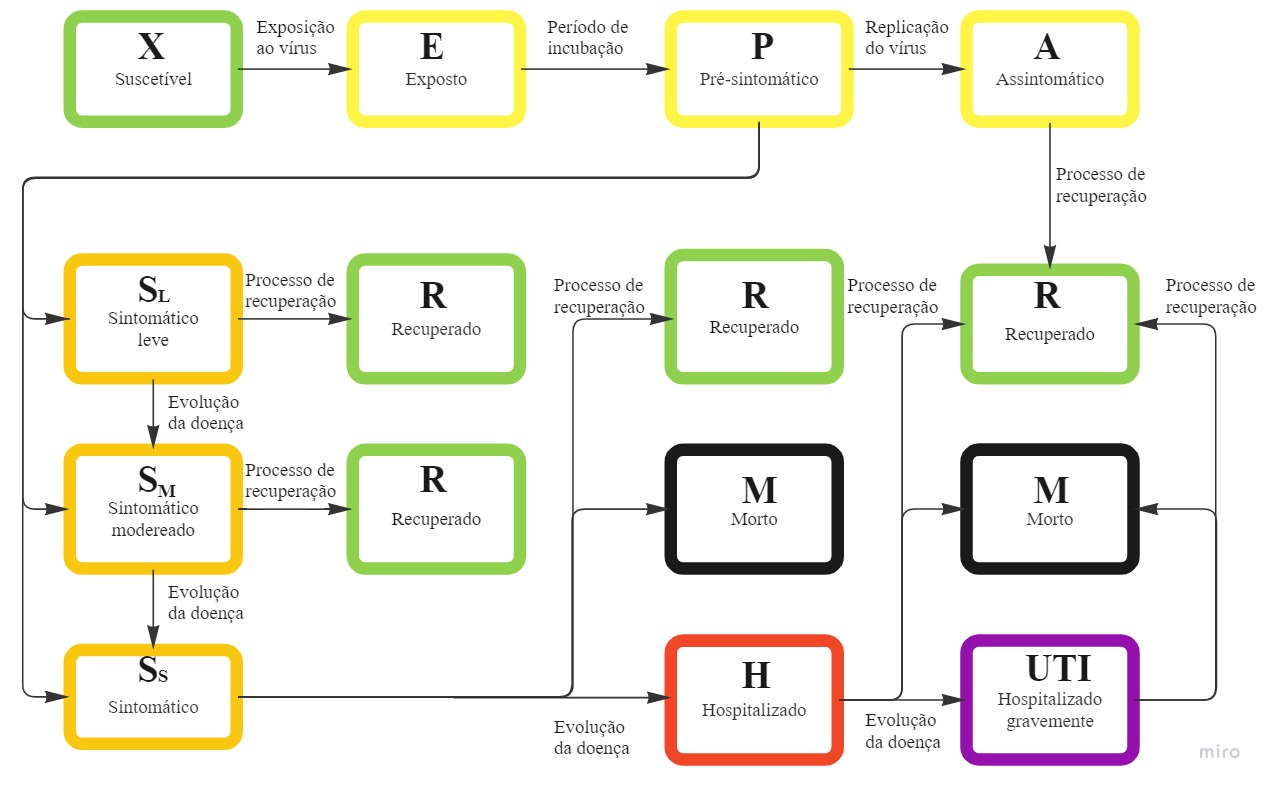
\includegraphics[width=0.9\textwidth]{Figures/covid fluxograma.jpg}
    \end{figure}

O indivíduo suscetível (X) entra em contato com o vírus e torna-se exposto (E), após o período de incubação torna-se pré-sintomático (P), a replicação do vírus ocorre e o indivíduo ou torna-se assintomático (A) e se recupera da doença, ou a doença evolui e o indivíduo se torna infeccioso, o indivíduo então pode ter sintomas leves ($S_l$), moderados ($S_m$) ou severos ($S_s$), caso não se recupere, será hospitalizado (H) e, em casos mais graves, internado em unidades de tratamento intensivo (UTI); na UTI o indivíduo ou se recupera, ou morre devido à doença.

No modelo, cada indivíduo ocupa uma posição em uma matriz quadrada de lado $L$ com população total $N = L \times L$, tal que $N$ é referente a cada cidade analisada. No início de cada simulação a população é iniciada com todos os indivíduos com estado suscetível (X), exceto 5 indivíduos que estarão em estado pré-sintomático, os indivíduos infectados entrarão em contato com sua vizinhança, Von Neumann para as cidades de baixa densidade populacional ou Moore para cidades de alta densidade, além dos contatos com outros indivíduos aleatórios. A probabilidade de infecção dos indivíduos suscetíveis é dada pela Equação \ref{eqn:prob}, um número aleatório $r$ é gerado e caso $r < P$, o indivíduo é infectado.

\section{Inicialização da população}

No início de cada simulação, além de receber o estado de saúde, cada indivíduo recebe uma idade atribuída de acordo com a estrutura etária da população brasileira, de modo que a distribuição de idades da rede reproduza a pirâmide etária real do país. A cada indivíduo é também atribuída uma idade de morte natural, sorteada por amostragem por rejeição a partir das probabilidades de morte natural por faixa etária, tal que a idade de morte respeita a expectativa de vida observada. Dessa forma, a rede inicia com uma população heterogênea em idade, o que é relevante uma vez que a evolução da Covid-19 e a sua letalidade dependem fortemente da faixa etária do indivíduo.

Os leitos de hospital e de UTI disponíveis para os doentes de Covid-19 são definidos a partir da razão de leitos por habitante de cada cidade, descontada a ocupação inicial de 50\% por outras doenças, de modo que apenas metade dos leitos esteja efetivamente disponível no início da simulação. A epidemia é iniciada com 5 indivíduos no estado pré-sintomático (P), distribuídos aleatoriamente na rede, enquanto os demais indivíduos permanecem suscetíveis.

\section{Dinâmica da simulação}

A simulação evolui em passos de tempo discretos, nos quais cada passo corresponde a um dia. A cada passo, antes de atualizar os estados, são aplicadas condições de contorno periódicas à rede, de modo que os indivíduos das bordas tenham como vizinhos os indivíduos da borda oposta, e logo a rede se comporta como uma superfície sem fronteiras, evitando efeitos de borda. Em seguida, percorre-se toda a rede e, para cada indivíduo, é aplicada a regra de transição correspondente ao seu estado de saúde atual, que determina o seu próximo estado. Por fim, a rede é atualizada de forma síncrona, ou seja, as transições calculadas para todos os indivíduos são aplicadas simultaneamente ao final do passo, de modo que a atualização de um indivíduo não interfira no cálculo dos demais no mesmo passo. O Algoritmo \ref{alg:simulacao} resume esse procedimento.

\begin{algorithm}[H]
\DontPrintSemicolon
\caption{Laço principal da simulação}
\label{alg:simulacao}
\For{cada simulação}{
  inicializa a população: estados de saúde, idades e leitos disponíveis\;
  \For{cada passo de tempo $t$ correspondente a um dia}{
    aplica as condições de contorno periódicas à rede\;
    \ForEach{indivíduo da rede}{
      aplica a regra de transição correspondente ao seu estado de saúde\;
    }
    atualiza a rede de forma síncrona\;
    substitui os indivíduos que sofreram morte natural por novos suscetíveis\;
    contabiliza a prevalência e a incidência de cada estado\;
  }
}
calcula a média das curvas sobre todas as simulações\;
\end{algorithm}

\subsection{Mecanismos de contágio}

A transmissão da doença ocorre por dois mecanismos complementares, ambos baseados na probabilidade de contágio dada pela Equação \ref{eqn:prob}. No primeiro mecanismo, cada indivíduo suscetível verifica a sua vizinhança e os seus contatos aleatórios, cujo número varia conforme a cidade, em busca de indivíduos infectados; o número de infectados encontrados, $n$, determina a probabilidade $P = 1 - (1 - \beta)^n$ de o suscetível ser infectado. No segundo mecanismo, cada indivíduo infectado, enquanto se encontra no período infeccioso, procura indivíduos suscetíveis entre seus contatos e tenta infectá-los, também de acordo com a probabilidade de contágio.

\begin{figure}[H]
\centering
\caption{Os dois mecanismos de contágio do modelo.}
\label{fig:contagio}
\begin{tikzpicture}[font=\small, >=Stealth,
   pessoa/.style={circle, draw, thick, minimum size=0.62cm, inner sep=0},
   susc/.style={pessoa, fill=green!18},
   infec/.style={pessoa, fill=red!55, text=white}]
  \begin{scope}
    \node[susc] (c1) at (0,0) {S};
    \node[infec] (a1) at (-1.2,0.9) {I};
    \node[susc]  (a2) at (1.2,0.9) {S};
    \node[infec] (a3) at (1.3,-0.5) {I};
    \node[infec] (a4) at (-1.1,-0.9) {I};
    \draw[->, dashed] (c1) -- (a1);
    \draw[->, dashed] (c1) -- (a2);
    \draw[->, dashed] (c1) -- (a3);
    \draw[->, dashed] (c1) -- (a4);
    \node[font=\footnotesize, align=center] at (0,-1.9) {(a) Suscetível busca\\ infectados};
  \end{scope}
  \begin{scope}[xshift=6cm]
    \node[infec] (c2) at (0,0) {I};
    \node[susc] (b1) at (-1.2,0.9) {S};
    \node[susc] (b2) at (1.2,0.9) {S};
    \node[susc] (b3) at (1.3,-0.5) {S};
    \node[susc] (b4) at (-1.1,-0.9) {S};
    \draw[->, thick] (c2) -- (b1);
    \draw[->, thick] (c2) -- (b2);
    \draw[->, thick] (c2) -- (b3);
    \draw[->, thick] (c2) -- (b4);
    \node[font=\footnotesize, align=center] at (0,-1.9) {(b) Infectado busca\\ suscetíveis};
  \end{scope}
\end{tikzpicture}
\end{figure}

Em (a), o indivíduo suscetível verifica a sua vizinhança e os seus contatos aleatórios em busca de infectados; em (b), o indivíduo infectado procura indivíduos suscetíveis entre seus contatos e tenta infectá-los. O segundo mecanismo é executado pelos estados pré-sintomático (P), assintomático (A) e sintomático leve ($S_l$), que representam os indivíduos infecciosos que ainda circulam na população, enquanto os estados sintomático moderado ($S_m$) e severo ($S_s$), por estarem afastados do convívio social, não procuram novos suscetíveis. Para evitar que um mesmo suscetível seja infectado duas vezes no mesmo passo de tempo, uma vez pela sua própria busca e outra por um infectado que o encontrou, utiliza-se um mecanismo de marcação que verifica se o indivíduo já foi contabilizado, garantindo a consistência da atualização.

\subsection{Transição entre estados e morte natural}

Cada estado de saúde possui uma duração, sorteada no momento em que o indivíduo entra no estado, dentro dos limites mínimo e máximo definidos para aquele estado (Tabela \ref{tab:dias}). Enquanto a duração não é atingida, o indivíduo permanece no mesmo estado; ao atingi-la, ocorre a transição para o próximo estado, que pode ser determinística ou sorteada de acordo com as probabilidades de transição (Tabela \ref{tab:prob}) e, em alguns casos, com a probabilidade de recuperação correspondente à faixa etária do indivíduo. A passagem para os estados de hospitalização (H) e de UTI depende ainda da disponibilidade de leitos, de modo que um indivíduo em estado severo só é hospitalizado se houver leito disponível.

Independentemente do estado de saúde, qualquer indivíduo pode sofrer morte natural ao atingir a sua idade de morte, situação na qual é removido e imediatamente substituído por um novo indivíduo suscetível, com idade sorteada novamente a partir da estrutura etária, de modo que o tamanho total da população permaneça constante ao longo da simulação.

\section{Parâmetros}

Para cada cidade a ser utilizada no modelo, a calibração da infecciosidade $\beta$ é necessária para que o valor de $R_0 = 3{,}5$ seja padrão em todas as cidades. É necessário também alterar os parâmetros que são específicos de cada cidade, são eles: tamanho da população, densidade populacional, contatos aleatórios, leitos de hospital e leitos de UTI, estes últimos obtidos a partir do Cadastro Nacional de Estabelecimentos de Saúde \cite{datasus}. A Tabela \ref{tab:area} mostra as características de quatro cidades: São Paulo (SP), Manaus (AM), Brasília (DF) e a favela da Rocinha (RJ).

\begin{table}[H]
\centering
\caption{Parâmetros de quatro diferentes áreas do Brasil.}
\label{tab:area}
\begin{tabular}{l c c c c c}
\hline
\textbf{Área} & \textbf{Densidade} & \textbf{L} & \textbf{Leitos/Pop} & \textbf{UTI/Pop} & \textbf{Contatos} \\
\hline
São Paulo & Alta  & 3355 & 0,00247452 & 0,00043782 & 2--19 \\
Rocinha   & Alta  & 264  & 0,00055111 & 0,00014592 & 2--120 \\
Brasília  & Baixa & 1604 & 0,00260879 & 0,00040114 & 2 \\
Manaus    & Baixa & 1343 & 0,00187124 & 0,00027858 & 2 \\
\hline
\end{tabular}
\end{table}

Já os parâmetros relacionados à doença são comuns a todas as áreas modeladas. A Tabela \ref{tab:dias} mostra a duração, em dias, do período de cada estado de saúde, e a Tabela \ref{tab:prob} mostra a probabilidade de transição entre os estados de saúde.

\begin{table}[H]
\centering
\caption{Parâmetros de duração de cada estado de saúde.}
\label{tab:dias}
\begin{tabular}{l l c}
\hline
\textbf{Parâmetro} & \textbf{Descrição} & \textbf{Duração (dias)} \\
\hline
$\tau_{l}$    & Período de latência   & 0--27 \\
$\tau_{P}$    & Pré-sintomático       & 0--14 \\
$\tau_{A}$    & Assintomático         & 0--7  \\
$\tau_{S_l}$  & Sintomático leve      & 0--14 \\
$\tau_{S_m}$  & Sintomático moderado  & 0--28 \\
$\tau_{S_s}$  & Sintomático severo    & 0--4  \\
$\tau_{H}$    & Hospitalização        & 7--45 \\
$\tau_{UTI}$  & UTI                   & 10--60 \\
\hline
\end{tabular}
\end{table}

\begin{table}[H]
\centering
\caption{Probabilidades de transição entre estados de saúde.}
\label{tab:prob}
\begin{tabular}{l l c}
\hline
\textbf{Parâmetro} & \textbf{Transição entre estados} & \textbf{Probabilidade} \\
\hline
$P_{(P\rightarrow A)}$    & Pré-sintomático para assintomático        & 0,5  \\
$P_{(P\rightarrow S_l)}$  & Pré-sintomático para sintomático leve     & 0,6  \\
$P_{(P\rightarrow S_m)}$  & Pré-sintomático para sintomático moderado & 0,2  \\
$P_{(P\rightarrow S_s)}$  & Pré-sintomático para sintomático severo   & 0,2  \\
$P_{(S_l\rightarrow S_m)}$ & Sintomático leve para sintomático moderado & 0,1 \\
$P_{(S_s\rightarrow H)}$   & Sintomático severo para hospitalização    & 0,75 \\
$P_{(S_s\rightarrow UTI)}$ & Sintomático severo para internação em UTI & 0,25 \\
\hline
\end{tabular}
\end{table}

\section{Estratégia de paralelização e validação}

A estratégia de paralelização adotada baseia-se no paralelismo de dados: uma vez que, a cada passo de tempo, todos os indivíduos da rede são processados de forma independente, associa-se uma thread a cada indivíduo, de modo que toda a rede é processada simultaneamente. A dinâmica da simulação é decomposta em kernels, um para cada estado de saúde, lançados em sequência a cada passo; como o lançamento de cada kernel funciona como um ponto de sincronização global, a ordem em que os estados são tratados na implementação serial é preservada. A geração de números aleatórios, por sua vez, é adaptada para a execução paralela, atribuindo-se um estado de gerador a cada thread. Em todas essas decisões, o princípio orientador é a preservação do comportamento do modelo, de modo que a implementação paralela reproduza os resultados da implementação serial.

Para que a paralelização seja considerada bem-sucedida, não basta que seja mais rápida; é necessário que produza os mesmos resultados da implementação serial, tomada como referência. A validação é feita comparando-se as curvas epidêmicas obtidas pelas duas implementações sob os mesmos parâmetros (mesma infecciosidade $\beta$, mesmo tamanho de rede e mesmo número de simulações), para cada uma das cidades modeladas. A concordância entre as curvas é quantificada pelo erro quadrático médio entre as proporções de cada estado ao longo do tempo, de modo que uma diferença pequena, compatível com a flutuação estatística do método de Monte Carlo, indica a equivalência entre as implementações.

Confirmada a equivalência, avalia-se o ganho de desempenho da implementação paralela. A avaliação é feita medindo-se a aceleração, definida no Capítulo \ref{FT} como a razão entre o tempo de execução da implementação serial e o da implementação paralela, e a eficiência correspondente, para cada cidade. Como as cidades possuem tamanhos de rede distintos, essa avaliação permite ainda observar como o ganho de desempenho varia com o tamanho do problema. A Figura \ref{fig:estrategia} resume a estratégia do trabalho.

\begin{figure}[H]
\centering
\caption{Estratégia do trabalho.}
\label{fig:estrategia}
\begin{tikzpicture}[font=\small, >=Stealth,
   bx/.style={draw, thick, rounded corners, align=center, minimum height=1cm, text width=3cm, fill=gray!8}]
  \node[bx, fill=blue!10] (modelo) at (0,0) {Modelo\\ (Capítulo \ref{Met})};
  \node[bx] (serial) at (-2.7,-2) {Implementação\\ serial (referência)};
  \node[bx] (gpu) at (2.7,-2) {Implementação\\ em GPU};
  \node[bx, fill=green!12] (valid) at (0,-4) {Validação\\ (mesmas curvas?)};
  \node[bx, fill=orange!15] (bench) at (0,-5.7) {Benchmark\\ (aceleração, eficiência)};
  \draw[->, thick] (modelo) -- (serial);
  \draw[->, thick] (modelo) -- (gpu);
  \draw[->, thick] (serial) -- (valid);
  \draw[->, thick] (gpu) -- (valid);
  \draw[->, thick] (valid) -- (bench);
\end{tikzpicture}
\end{figure}

O mesmo modelo é realizado em duas implementações; a implementação em GPU é validada contra a serial sob os mesmos parâmetros e, confirmada a equivalência, avalia-se o seu desempenho.
